%-----------------------------------------------------------------------------80
% SECTION TITLE|
%-----------------------------------------------------------------------------80

\section{Estructura de un programa en Fortran}

%-----------------------------------------------------------------------------80
% CONTENT
%-----------------------------------------------------------------------------80
%Definición-------------------------------------------------------------------80

\subsection{Programa en Fortran}
\begin{frame}[fragile]{Estructura de un programa en Fortran}
  \begin{itemize}[<+(1)->]
   \item Un programa en Fortran está ordenado lógica y jerarquicamente en unidades programáticas. 
   \item Tiene una unidad principal, llamada programa principal, la cual contiene las instrucciones que definen el objetivo del programa.
   \item Es posible recurrir a subprogramas, que agrupados constituyen una instrucción del programa principal. 
   \item [] 
   
   \begin{minted}[linenos,autogobble]{fortran}
PROGRAM         ejemplo   !nombre del programa          !sentencia no ejecutable
IMPLICIT NONE             !declara todas las variables  !sentencia no ejecutable                               
INTEGER         i         !declaración variables        !sentencia no ejecutable
                i = 3     !código del programa          !sentencia ejecutable
WRITE(*,*)      ’ i =’,i  !código del programa          !sentencia ejecutable
END PROGRAM ejemplo                                     !sentencia ejecutable
  \end{minted}
\end{itemize} 
\end{frame}

\begin{frame}[fragile]{Estructura de un programa en Fortran}
 \begin{figure}
  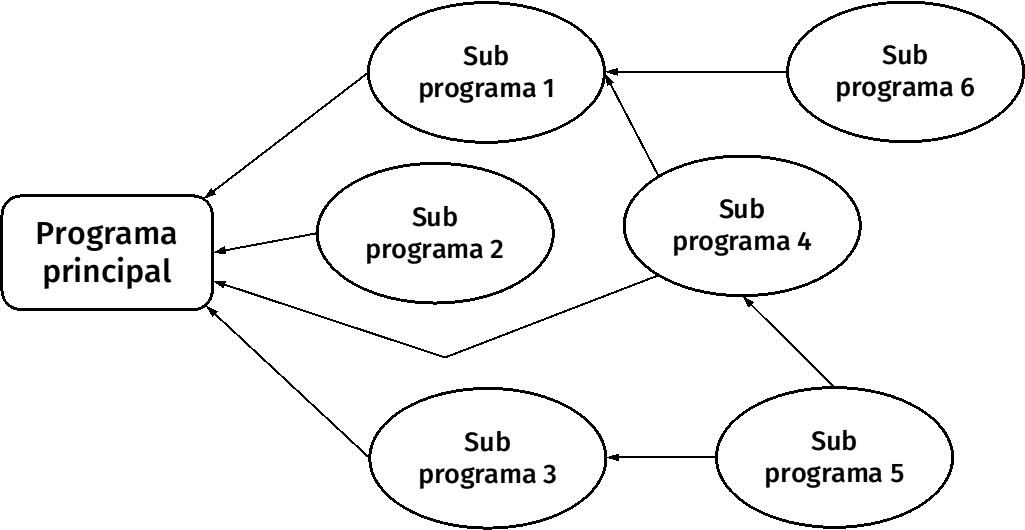
\includegraphics[width=1\textwidth]{./resources/structurep.png}
  \caption{Esquema de la estructura de un programa en Fotran}
 \end{figure}
\end{frame}